%======================================================================
% Poznamky_2_variacni_metody.pdf
%======================================================================
\section{Ritzův variační princip}
\strana{VP-1}

Střední hodnota energie ve stavu $\ket{\psi}$ je
\[
  \vzorec{E[\psi] \equiv \langle H\rangle_\psi = \frac{\mel{\psi}{H}{\psi}}{\braket{\psi}{\psi}}} \qquad\text{(RVP)}
\]
Podívejme se na změnu $E$ při záměně $\ket{\psi}\to\ket{\psi} + \ket{\delta\psi}$
\begin{align*}
  \delta E \equiv E[\psi + \delta\psi] - E[\psi]
  &= \frac{\mel{\psi}{H}{\psi} + \mel{\delta\psi}{H}{\psi} + \mel{\psi}{H}{\delta\psi}}{\braket{\psi}{\psi} + \braket{\delta\psi}{\psi} + \braket{\psi}{\delta\psi}} - E + O(\|\delta\psi\|^2) \\
  &= \frac{\mel{\delta\psi}{H - E}{\psi} + \mel{\psi}{H - E}{\delta\psi}}{\braket{\psi}{\psi} + \braket{\delta\psi}{\psi} + \braket{\psi}{\delta\psi}} + O(\|\delta\psi\|^2)
\end{align*}
Stacionární hodnoty funkcionálu (RVP) $\Leftrightarrow$
\[
  \mel{\delta\psi}{H - E}{\psi} + \mel{\psi}{H - E}{\delta\psi} = 0 \qquad \forall\ket{\delta\psi}
\]
splněno $\forall\ket{\delta\psi}$, tj.\ i pro $i\ket{\delta\psi}$:
\[
  \times(\pm i)\,\big| \qquad -i\mel{\delta\psi}{H - E}{\psi} + \mel{\psi}{H - E}{\delta\psi}\,i = 0
\]
\[
  \Rightarrow\qquad \mel{\delta\psi}{H - E}{\psi} = \mel{\psi}{H - E}{\delta\psi} = 0 \qquad \forall\ket{\delta\psi}
\]

\begin{veta}[Tvrzení 1]
Funkcionál (RVP) nabývá stacionárních hodnot pro stacionární stavy $H\ket{\psi_n} = E_n\ket{\psi_n}$. \quad \dots\ $E[\ket{\psi_n}]$ \dots\ stac.\ hodnota.
\end{veta}

\underline{Důsledek:} Pokud nějak odhadneme $\ket{\tilde\psi_n} = \ket{\psi_n} + \ket{\delta\psi}$, tak \kw{chyba ve výpočtu energie je druhého řádu} v $\|\delta\psi\|$.

\underline{Poznámka:} Striktně řečeno výroky
\begin{align*}
  \mel{\delta\psi}{H - E}{\psi} &= 0 \quad \forall\ket{\delta\psi} && \text{(V1)} \\
  \text{a}\quad (H - E)\ket{\psi} &= 0 && \text{(V2)}
\end{align*}
nejsou ekvivalentní, respektive $\mel{\delta\psi}{H - E}{\psi}$ lze vyčíslit pro větší třídu funkcí. (V1) se nazývá \kw{\uv{SLABOU FORMULACÍ}} úlohy (v tomto případě S.R.). Kinetický člen (pro částici v potenc.\ poli):
\begin{align*}
  \mel{\delta\psi}{H}{\psi} &= -\frac{\hbar^2}{2m}\int\delta\psi(\vec r)^*\,\Delta\psi(\vec r)\,\dd^3\vec r + \int\delta\psi(\vec r)^*V(\vec r)\psi(\vec r)\,\dd^3\vec r \\
  &\overset{\text{per partes}}{=} \frac{\hbar^2}{2m}\int(\nabla\delta\psi)^*\cdot\big(\nabla\psi(\vec r)\big)\,\dd^3\vec r + \int\delta\psi(\vec r)^*V(\vec r)\psi(\vec r)\,\dd^3\vec r
\end{align*}
$\uparrow$ tato forma je matematicky výhodná \dots\ nemusí $\exists$ druhé derivace $\psi$ \\
\dots\ Sobolevovy prostory \dots

%----------------------------------------------------------------------
\strana{VP-2}
\begin{veta}[Tvrzení 2]
Nechť $E_0$ je energie základního stavu pro $\hat H$. Potom
\[
  \vzorec{E_0 \leq E[\psi] \equiv \frac{\mel{\psi}{\hat H}{\psi}}{\braket{\psi}{\psi}}} \qquad \forall\ket{\psi}
\]
\end{veta}

\underline{Důkaz:}
\[
  E[\psi] = \frac{\sum_n E_n|\braket{n}{\psi}|^2}{\sum_n|\braket{n}{\psi}|^2} \geq \frac{E_0\sum_n|\braket{n}{\psi}|^2}{\sum_n|\braket{n}{\psi}|^2} = E_0
\]
+ je vidět \dots\ rovnost $\Leftrightarrow$ $\ket{\psi}$ patří do vl.\ podprostoru $\hat H$ příslušného $E_0$.

\underline{Použití:} Určitá třída \kw{testovacích funkcí} $\ket{\psi(\alpha_1,\alpha_2,\dots,\alpha_n)}$ \\
\quad $E[\psi(\alpha_1\dots\alpha_n)]$ je funkce parametrů $\alpha_1\dots\alpha_n$ + hledáme min. \\
\quad tj.\ $\dfrac{\partial E}{\partial\alpha_i} = 0\ \ \forall\alpha_i$ \quad \dots\ minimum v $\vec\alpha = \vec\alpha^{(0)} \equiv (\alpha_1^{(0)}\dots\alpha_n^{(0)})$ \\
\quad pak $\ket{\psi(\alpha^{(0)})}$ je aproximace vln.\ fce zákl.\ stavu a $E[\psi(\alpha^{(0)})]$ je \kw{horní odhad energie}.

\underline{Pozn:} lze zkonstruovat i dolní odhad (viz Ballentine)

\underline{Speciální případ:} třída testovacích funkcí tvoří podprostor:
\[
  \ket{\psi} = \alpha_1\ket{\phi_1} + \alpha_2\ket{\phi_2} + \dots + \alpha_n\ket{\phi_n}
\]
\[
  \text{(V1)}\ \Rightarrow\ \sum_{ij}\delta\alpha_i^*\mel{\phi_i}{H}{\phi_j}\alpha_j - E\sum_{ij}\delta\alpha_i^*\braket{\phi_i}{\phi_j}\alpha_j = 0 \qquad \forall\delta\alpha_i
\]
\[
  \text{tj.}\qquad \vzorec{\sum_j\Big[\mel{\phi_i}{H}{\phi_j} - E\braket{\phi_i}{\phi_j}\Big]\alpha_j = 0} \qquad \forall i
\]
zobecněná rovnice pro vl.\ č.\ matice \quad \pozn{vl.\ č.\ $\det\{\mathcal{H} - E\mathcal{S}\} = 0$}
\begin{itemize}
  \item speciálně pro ON-bázi $\braket{\phi_i}{\phi_j} = \delta_{ij}$ \quad $\to\ \sum_j\mathcal{H}_{ij}\alpha_j = E\alpha_i$ \\
        $\to$ vlastní čísla a vl.\ vektory matice $\mathcal{H}_{ij} \equiv \mel{\phi_i}{\hat H}{\phi_j}$
  \item v obecném případě je třeba nejdříve diagonalizovat matici $\mathcal{S}_{ij} = \braket{\phi_i}{\phi_j} = U^\dagger\Lambda U$ \\
        \dots\ \kw{Löwdinova symetrická ortogonalizace}
\end{itemize}
\pozn{$H\ket{\psi} = E\,S\ket{\psi}$ \ $\to$ \ $\underbrace{\tfrac{1}{\sqrt S}H\tfrac{1}{\sqrt S}}_{\tilde H}\cdot\underbrace{\sqrt S\ket{\psi}}_{\ket{\tilde\phi}} = E\cdot\sqrt S\ket{\psi}$, \quad $\tilde H\ket{\tilde\phi} = E\ket{\tilde\phi}$}

%----------------------------------------------------------------------
\strana{VP-3}
\begin{veta}[Tvrzení 3 (Hylleraas--Undheim theorem)]
Nechť $E_0\leq E_1\leq E_2\leq\dots$ jsou přesné vl.\ č.\ $\hat H$ (každé tolikrát, kolik je jeho násobnost) \\
a nechť $\varepsilon_0\leq\varepsilon_1\leq\varepsilon_2\leq\dots$ jsou vl.\ č.\ problému $\det\{\mathcal{H} - \varepsilon\mathcal{S}\} = 0$.

Potom: \qquad $\vzorec{E_i \leq \varepsilon_i} \qquad \forall i = 1,\dots N$ \quad \dots\ (dimenze podprostoru test.\ fcí)
\end{veta}

\underline{Náznak důkazu:}

\begin{minipage}{0.55\textwidth}
Postupně přidáváme řádky a sloupce matice:
\end{minipage}
\begin{minipage}{0.4\textwidth}
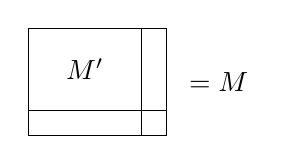
\begin{tikzpicture}[scale=0.8]
  \draw (0,0) rectangle (2.2,1.7);
  \draw (0,0.4) -- (2.2,0.4);
  \draw (1.8,0) -- (1.8,1.7);
  \node at (0.9,1.05) {$M'$};
  \node[right] at (2.4,0.85) {$= M$};
\end{tikzpicture}
\end{minipage}

\begin{minipage}{0.3\textwidth}
dá se DK, že
\end{minipage}
\begin{minipage}{0.4\textwidth}
\begin{tikzpicture}[x=1cm,y=0.45cm,>=Stealth]
  % levý sloupec: lambda' (M'), pravý sloupec: lambda (M)
  \foreach \y in {4.5,3,1.5,0} \draw (0,\y) -- (0.5,\y);
  \foreach \y in {5.2,3.8,2.3,0.8,-0.6} \draw (2,\y) -- (2.5,\y);
  \node[left] at (0,4.5) {$\lambda'_{N-1}$};
  \node[left] at (0,0) {$\lambda'_1$};
  \node[left] at (0,2.25) {$\vdots$};
  \node[right] at (2.5,5.2) {$\lambda_N$};
  \node[right] at (2.5,-0.6) {$\lambda_1$};
  \node[right] at (2.5,2.3) {$\vdots$};
  \draw[->] (0.5,3) -- (2.6,2.0);
  \draw[->] (0.5,1.5) -- (2.6,0.5);
  \draw[->] (0.5,0) -- (2.6,-0.9);
\end{tikzpicture}
\end{minipage}
\begin{minipage}{0.25\textwidth}
\dots\ navzájem se dělí
\end{minipage}

\noindent\rule{3cm}{0.4pt}

DK, že se navzájem dělí \dots\ najdeme bázi, v níž $M'$ diagonální
\[
  \to\quad M = \left(\begin{array}{ccc|c}
    \lambda'_1 & & & M_{1N} \\
    & \ddots & & \vdots \\
    & & \lambda'_{N-1} & \\ \hline
    M_{N1} & \cdots & & M_{NN}
  \end{array}\right)
  \quad\dots\quad
  f(\lambda) \equiv \det(M - \lambda\hat I)
\]
\[
  f(\lambda) = (M_{NN} - \lambda)\prod_{n=1}^{N-1}(\lambda'_n - \lambda) - \sum_{m=1}^{N-1}|M_{mN}|^2\prod_{n\neq m}(\lambda'_n - \lambda)
\]
$f(\lambda)$ je char.\ polynom. Vyčíslený v $\lambda = \lambda'_k$:
\[
  f(\lambda'_k) = -|M_{kN}|^2\prod_{n\neq k}(\lambda'_n - \lambda'_k)
  \quad\to\quad \text{střídá znaménko pro } k = 1,2,\dots
\]
\hfill $+\ f(\lambda\to-\infty)\to+\infty$, \quad $f(\lambda\to+\infty)\to(-1)^N\infty$

\noindent\rule{3cm}{0.4pt}

\textbf{Poznámky:}
\begin{itemize}
  \item Základní způsob použití $\to$ základní stav jako minimum (i nelineární test.\ prostor)
  \item Excitované stavy, ale základní pro danou symetrii \dots\ jako $\uparrow$ \\
  \begin{minipage}[t]{0.5\textwidth}
    PŘ: sudé a liché fce: \quad
    $H = \left(\begin{array}{c|c} H_S & 0 \\ \hline 0 & H_L\end{array}\right)$
  \end{minipage}
  \begin{minipage}[t]{0.45\textwidth}\raggedright
    sfér.\ sym.\ potenciál \\
    $H = \begin{pmatrix} \boxed{H_0} & & 0 \\ & \boxed{H_1} & \\ 0 & & \ddots\ \boxed{H_l}\end{pmatrix}$
  \end{minipage} \\
  + složitější \dots\ sym.\ molekul, krystalů \dots\ teorie grup.
  \item Netriviální excitace $\to$ Hylleraas--Undheim \dots\ max; + stac.\ stav.
  \item souvislost s poruchovou teorií: \quad $H = H_0 + H_1$ \\
        \dots\ pro hledání $E_0$ použijeme test.\ prostor $\ket{\phi_k} = \ket{n=0,k}$ \\
        $\to$ korekce 1.\ ř.\ $=$ vl.\ č.\ $\mel{0,m}{H_1}{0,k}$ \dots\ totožné s variačním principem. \\
        (konzist.\ s tím, že korekce 2.\ ř.\ je vždy $< 0$) \quad $\Rightarrow$ horní odhad!
\end{itemize}

%----------------------------------------------------------------------
\strana{VP-4}
\subsection*{Dolní odhad?}
nechť $\ket{\psi}$ je odhad vl.\ fce pro $E_n$ (normovaná) \\
\dots\ def \quad $\varepsilon \equiv \mel{\psi}{H}{\psi}$ \quad a zbytek \quad $\ket{R} \equiv (H - \varepsilon)\ket{\psi}$ \\
pak
\[
  \braket{R}{R} = \mel{\psi}{(H - \varepsilon)^2}{\psi} = \sum_{n'}|\braket{n'}{\psi}|^2(E_{n'} - \varepsilon)^2
  \underset{\uparrow}{\geq} (E_n - \varepsilon)^2\underbrace{\sum_{n'}|\braket{n'}{\psi}|^2}_{=1}
\]
odhad, ale musíme něco vědět! (nebo doufat) $\to$ \pozor{za předp.\ $E_n$ je nejbližší vl.\ č.\ k hodnotě $\varepsilon$!}

pak \quad $\to$ \quad $\vzorec{\varepsilon - \Delta \leq E_n \leq \varepsilon + \Delta}$ \quad kde \quad $\Delta \equiv \sqrt{\braket{R}{R}}$

lepší odhady: je třeba vědět více o spektru $\to$ viz Ballentine

\begin{priklad}[PŘÍKLADY: Atom vodíku (Ballentine)]
\[
  H = \underbrace{\frac{p^2}{2\mu}}_{K} \underbrace{-\ \frac{e^2}{r}}_{+P}; \qquad
  \psi(r) = e^{-r/a} \qquad N = \braket{\psi}{\psi} = \pi a^3 = \int|\psi|^2\dd^3r
\]
\pozn{přesné $\psi = \frac{1}{\sqrt{\pi a_0^3}}e^{-r/a}$ $\leftarrow$ normované}
\begin{align*}
  \to\quad K &= \frac{\hbar^2\pi a}{2\mu}
     = \frac{\hbar^2}{2\mu}\cdot\frac{4\pi}{a^2}\int_0^\infty e^{-2r/a}r^2\,\dd r
     = \frac{\hbar^2}{2\mu}\int\Big|\frac{\partial\psi}{\partial r}\Big|^2\dd^3r \\
  P &= -\pi e^2a^2 = -e^2\,4\pi\int_0^\infty e^{-2r/a}r\,\dd r = -\int|\psi|^2\frac{e^2}{r}\,\dd^3r
\end{align*}
tj.\ \quad $\langle H\rangle = \dfrac{K + P}{N} = \dfrac{\hbar^2}{2\mu a^2} - \dfrac{e^2}{a}$
\quad $\to$ \quad min.\ pro \quad $\vzorec{a = \frac{\hbar^2}{\mu e^2}}$

\underline{Srovn:}
\[
  \begin{array}{c|ccc}
    \psi = & Ce^{-r/a} & \dfrac{C}{r^2 + a^2} & Cre^{-r/a} \\[6pt] \hline
    \rule{0pt}{14pt}\dfrac{\langle H\rangle}{E_0} = & -1 & -0.81 & -0.75 \\[6pt]
    1 - |\braket{\psi}{100}|^2 & 0 & 0.21 & 0.05
  \end{array}
\]
\dots\ tj.\ \pozor{lepší vln.\ fce neznamená lepší energii!}
\end{priklad}
